\chapter{Metodologia pracy}
\section{Budowa i konfiguracja klastra}

Klaster obliczeniowy stanowi zespół komputerów połączonych w ten sposób, by prowadzić równolegle obliczenia, dzięki czemu czas potrzebny na ich wykonanie ulega skróceniu w porównaniu do pojedynczej jednostki obliczeniowej. Dzięki temu uzyskujemy wzrost wydajności bez potrzeby oczekiwania na coraz to nowszy sprzęt.

Budowany klaster składał się z dwóch dwuprocesorowych jednostek centralnych Dell Precision T5500, z czego każdy procesor posiadał 4 rdzenie. Razem daje to możliwość uruchomienia 16 niezależnych procesów. Specyfikacja sprzętu przedstawiona została w tabeli 4.1.

\begin{table}[ht!]
\centering
  \begin{tabular}{| r | p{10cm} |}
  \hline
  Podzespół & Opis \\
  \hline
 Procesor &  2 $\times$ Intel® Xeon® E5630; 4 rdzenie; 64 bit; taktowanie 2.53 GHz; 12 MB Cache \\
 Płyt główna & Intel® 5520 chipset; dwuprocesorowa\\
 Pamięć RAM & 12 GB; DDR3\\
 Dysk twardy & 500 GB; SATA\\
 karta sieciowa & Dwie karty sieciowe 1Gbps; jedna wbudowana na płycie głównej, druga w gnieździe PCI\\
 \hline  
  \end{tabular}
  \caption{Specyfikacja komputerów.}
\end{table}
Każdy z procesorów posiadał opcję HyperThreding, co pozwala na wirtualne podwojenie liczny rdzeni, jednak wcześniejsze obliczenia programem Gromacs pokazały, że włączenie opcji HT nie zwiększa wydajności obliczeń, a może ją wręcz zmniejszać w wyniku zwiększenia komunikacji pomiędzy wątkami przy dotychczasowej przepustowości.

Aby fizycznie zbudować klaster wystarczyło połączyć komputery do jednej sieci Ethernet za pomocą switcha (ośmioportowy D-link DGS-1008D 1000Mbps). Na tak połączonych komputerach należało następnie zainstalować system operacyjny. Ze względu na fakt, że pakiet Gromacs był domyślnie pisany pod systemy Uniksowe oraz rozpowszechnienie na pracowni wybór padł na system Ubuntu w serwerowej wersji 10.04 LTS (64 bit). Ponadto system ten jest darmowy oraz dobrze udokumentowany. Następnym etapem była instalacja bibliotek niezbędnych do działania Gromacsa na każdym z komputerów.

\subsection{Instalacja biblioteki OpenMPI}

Przy obliczeniach równoległych podstawowym problemem jest komunikacja pomiędzy poszczególnymi procesami (węzłami) klastra. W celu ułatwienia tworzenia programów działających równolegle stworzono na początku lat dziewięćdziesiątych protokół komunikacji \textbf{MPI} (ang. Message Passing Interface), który ze względu na rozpowszechnienie stał się standardem i występuje w postaci bibliotek dla różnych języków programowania i systemów operacyjnych. Protokół ten jest odpowiedzialny między innymi za zarządzanie pamięcią, synchronizację danych, komunikację pomiędzy procesami oraz rozdział procesów na poszczególne węzły. 

Również Gromacs korzysta ze standardu MPI. W związku z czym potrzebna była instalacja bibliotek obsługujących ten standard. Ze względu na rozpowszechnienie oraz na częste aktualizacje i szybkie poprawianie błędów wybrano bibliotekę OpenMPI w wersji 1.4.2, która dystrybuowana jest na licencji Open Source, dzięki czemu jest darmowa. Instalacja polega na ściągnięciu oraz rozpakowaniu archiwum z kodem źródłowym bibliotek, konfiguracji oraz kompilacji. Przy domyślnie zainstalowanym systemie instalacja sprowadza się do wykonania 3 podstawowych poleceń.
\begin{enumerate}
\item \texttt{./configure} -- uruchomienie skryptu konfiguracyjnego
\item \texttt{make} -- kompilacja
\item \texttt{make install} -- instalacja
\end{enumerate}
Przy konfiguracji należy pamiętać, by jako domyślną ścieżkę instalacji bibliotek podać katalog systemowy \texttt{/usr/lib}, po czym instalację wykonywać przy uprawnieniach superużytkownika (\texttt{sudo make install}). Dzięki temu uniknie się problemów przy dostępie do tych bibliotek przez inne programy i innych użytkowników.


\subsection{Instalacja biblioteki FFTW}
Kolejnym krokiem jest instalacja bibliotek do wykonywania transformaty Fourierowskiej. Ze względu na szybkość największą popularnością cieszy się biblioteka FFTW. Pomimo dostępności w repozytorium systemu Ubuntu zaleca się kompilację ze źródeł, ponieważ dzięki temu uwzględnia się wszystkie możliwe optymalizacje dostępne pod dany procesor, a nie tylko te najbardziej uniwersalne.

Do instalacji użyto biblioteki FFTW w wersji 3.2.2. Instalacja przebiega podobnie jak w przypadku OpenMPI. Domyślnie biblioteka ta kompiluje się w podwójnej precyzji, kiedy większość obliczeń Gromacsem odbywa się w pojedynczej precyzji, przez co podwójna precyzja biblioteki FFTW nie jest potrzebna. 

Kompilację i instalację prowadzi się przez wykonanie skryptu \texttt{./configure} z opcją \texttt{--enable-single}. Dzięki temu kompiluje się tę bibliotekę w pojedynczej precyzji. Ponadto można uwzględnić opcję obliczeń wielowątkowych dla systemów wielordzeniowych \texttt{--enable-threads} oraz instrukcje SSE dla rodziny procesorów i686 i nowszych \texttt{--enable-sse}.

Do poprawnej komunikacji pomiędzy programami wykorzystującymi bibliotekę OpenMPI na różnych komputerach wymagana jest możliwość zdalnego wywoływania poleceń na wszystkich komputerach wchodzących w skład klastra. Do tego celu służy protokół SSH (ang. \textit{Secure Shell}). Do obsługi wymagana jest instalacja serwera SSH na każdym z komputerów oraz możliwość bezhasłowego logowania się pomiędzy tymi węzłami. 

\subsection{Instalacja programu Gromacs}

Przy symulacjach użyto programu Gromacs w wersji 4.5.1. Jego instalacja jest zbliżona do instalacji bibliotek, jednak przy konfiguracji należy podać odpowiednie parametry do uzyskania wersji obsługującej obliczenia równoległe.

Dogodnie jest wykonać dwie instalacje. Jedną dla wersji bez obsługi protokołu MPI, a drugą z obsługą. Pierwszą instalację konfiguruje się standardowym skryptem \texttt{./configure} z podaniem ścieżki instalacji oraz wyborem zainstalowanej wersji bibliotek do transformaty fourierowskiej, w tym przypadku FFTW \texttt{--enable-fft=fftw3}. Całość kompiluje się poleceniem \texttt{make} oraz instaluje poleceniem \texttt{sudo make install} jeśli potrzeba, by program był dostępny dla wszystkich użytkowników oraz podana ścieżka instalacji nie znajduje się w katalogu użytkownika.

Aby dodać obsługę MPI przy konfiguracji należy podać opcję \texttt{--enable-mpi}. Aby rozróżnić instalację Gromacsa z MPI należy przy konfiguracji uwzględnić opcję, która do nazwy programu z obsługą MPI doda sufiks \_mpi \texttt{--program-suffix=\_mpi}. 

Poza głównym programem odpowiedzialnym za symulacje dynamiki pozostałe programy pakietu Gromacs nie korzystają z obsługi MPI, w związku z czym wystarczy skompilować i zainstalować tylko \texttt{mdrun} z obsługą MPI. Po konfiguracji służą do tego polecenia \texttt{make mdrun} oraz \texttt{sudo make install-mdrun}.

\section{Przygotowanie struktury do symulacji}
Jako przygotowanie cząsteczki do symulacji rozumie się wszelkie działania na plikach, podczas których nie wykonujemy obliczeń symulacji dynamiki molekularnej, które należy jednak przeprowadzić w celu uzyskania prawidłowej struktury wejściowej. Proces ten można rozbić na kilka najczęściej występujących etapów:
\begin{itemize}
\item Konwersja struktury na wewnętrzny format Gromacsa
\item Umieszczenie cząsteczki w pudełku
\item Dodatek wody do układu
\item Dodatek jonów do układu
\end{itemize}

Aby przeprowadzić symulację dynamiki danej cząsteczki należy dysponować jej strukturą, którą uzyskuje się w wyniku badań krystalograficzncyh lub NMR. W internecie istnieje otwarta i darmowa baza danych z rozwiązanymi strukturami białek, RCSB Protein Data Bank \cite{pdbdb}, z której można pobrać plik w formacie PDB.

Jeśli badane białko zawiera aminokwasy kwasowe bądź zasadowe, to należy pamiętać, że różne stany sprotonowania prowadzą do różnej struktury, co może mieć wpływ na otrzymane wyniki. W celu optymalizacji struktury należy posłużyć się programem WHATIF, który jest dostępny w postaci usługi sieciowej z poziomu przeglądarki internetowej \cite{WHATIF}. W pliku PDB zawierającym definicję białka 1TKI należało ręcznie usunąć linie zawierające wpisy położeń wody krystalizacyjnej oraz jednego z dwóch łańcuchów.

Posiadając już odpowiedni plik PDB należy przekonwertować go na wewnętrzny format używany przez Gromacsa. Do tego celu służy jeden z programów pakietu Gromacs, mianowicie \textsf{pdb2gmx}. W wyniku jego działania otrzymujemy plik \texttt{.gro} zawierający informacje o wielkości pudła, liczbie atomów w układzie, ich położeniach i prędkościach oraz plik z topologią \texttt{.top}, w którym znajdują się definicje typów atomów, ich masy, ładunki, typy wiązań oraz definicje oddziaływań i odwołania do pól siłowych.

Pole siłowe stanowi bazę zawierającą definicje dla ładunków cząstkowych atomów, długości wiązań, ich stałych siłowych, oraz innych oddziaływań dla różnego typu cząsteczek (ang. \textit{residues}) takich jak aminokwasy, nukleotydy, cukry czy też parametry dla jonów. W zależności od dokładności definicji atomów pola siłowe dzielimy na pola typu \textit{all atom}, które zawierają definicje dla ładunków oraz oddziaływań dla wszystkich atomów występujących w cząsteczce oraz na pola typu \textit{united atom}, które pomijają definicje dla atomów wodorów niepolarnych. Jeśli zamierza się symulować dynamikę cząsteczek nieujętych w definicji pola siłowego należy uzyskać na podstawie obliczeń kwantowomechanicznych ładunki cząstkowe oraz parametry dla oddziaływań w cząsteczce i dodać tę definicję. Komplikuje to używanie programów \textbf{MD} do niestandardowych układów.

Program używany do konwersji, \texttt{pdb2gmx} pozwala na wybór pola siłowego, modelu wody oraz stanu sprotonowania poszczególnych aminokwasów. Do symulacji użyto pola siłowego GROMOS, które jest polem typu \textit{united atom} oraz modelu wody SPC. Stany sprotonowania histydyn zostały wybrane w oparciu o strukturę w pliku PDB otrzymanego w wyniku użycia programu WHATIF. Program ten dodaje również atomy wodoru nie wykryte podczas ustalania struktury. Wybrane pole siłowe nie zawiera definicji wszystkich atomów wodorów występujących w strukturze w pliku PDB, co prowadzi do błędów podczas konwersji na format plików Gromacsa. Aby temu zapobiec stosuje się program \texttt{pdb2gmx} z opcją \texttt{-ignh}, która powoduje pobranie informacji o położeniach atomów wodoru nie z pliku PDB, ale z definicji pola siłowego. Dodatkowa opcja \texttt{-his} pozwala na interaktywny wybór stanu sprotonowania histydyny, dzięki czemu informacja o wodorach biorących udział w tworzeniu wiązań wodorowych nie jest tracona.

Aby zdefiniować rozmiary pudełka wykorzystuje się kolejny z programów Gromacsa, \texttt{editconf}. Początkowe wymiary pudełka obieramy na podstawie publikacji\cite{1tki} na 8.8 x 7.8 x 7.6 nm. Białko umieszcza się w pudełku poleceniem \texttt{editconf} z parametrami pliku wejściowego, wyjściowego oraz opcją \texttt{-box 8.8 7.8 7.6} określającą wymiary w nm oraz \texttt{-c} umieszczającą środek geometryczny białka w środku pudełka.

Kolejnym etapem jest dodatek cząsteczek wody do układu. Gromacs zawiera zdefiniowane kilka różniących się od siebie modeli wody:
\begin{itemize}
\item \textbf{SPC} --- prosty, trójpunktowy model wody
\item \textbf{SPC/E} --- rozszerzony trójpunktowy model wody
\item \textbf{TIP3P} --- trójpunktowy model wody stosowany w polach siłowych CHARMM i AMBER
\item \textbf{TIP4P} --- czteropunktowy model wody, gdzie 3 punkty stanowią atomy tlenu i wodoru, natomiast czwarty punkt stanowi zdelokalizowany ładunek. Stosowany najczęściej dla pola siłowego OPLS/AA
\item \textbf{TIP5P} --- model pięciopunktowy, gdzie dwa dodatkowe punkty odpowiadają definicjom wolnych par elektronowych tlenu
\end{itemize}
Chcąc powtórzyć wyniki pracy \cite{1tki} wybrano model SPC.

Do addycji wody do układu służy program \texttt{genbox}. W linii poleceń oprócz pliku wejściowego, wyjściowego oraz pliku z topologią należy podać plik ze strukturą wody, która zostanie powielona. W tym przypadku definicje wody znajdują się w pliku \texttt{spc216.gro} znajdującym się w katalogu głównym Gromacsa. W wyniku działania programu otrzymuje się układ składający się z 49606 atomów. 

Następnie należało dodać do układu jony w celu zrównoważenia ładunku +2e białka oraz aby zbliżyć układ do warunków eksperymentalnych. Wykorzystuje się do tego program \texttt{genion}, będący częścią składową Gromacsa. Przed jego użyciem należy posiadać plik wsadowy do symulacji \texttt{.tpr}, który generuje się komendą \texttt{grompp}. Jako plik z parametrami posłużył plik do minimalizacji energii \texttt{em.mdp}. Posiadając już plik wsadowy należy w poleceniu \texttt{genion} podać go jako plik wejściowy, podać plik wyjściowy, plik z topologią oraz opcją \texttt{-nn} liczbę jonów ujemnych oraz \texttt{-np} liczbę jonów dodatnich. Jako domyślne program ten bierze kationy sodu oraz aniony chlorkowe, których liczba wynosi odpowiednio 29 i 27.

Istnieje również możliwość ustalenia stężenia jonów za pomocą opcji \texttt{-conc} w mol/litr oraz opcji \texttt{-neutral}, która odpowiada za otrzymanie układu elektrycznie obojętnego.

Mając tak zdefiniowany układ można przejść do właściwego etapu, jakim jest symulacja.

\section{Równowagowanie}

\begin{figure}[h!]
\begin{centering}
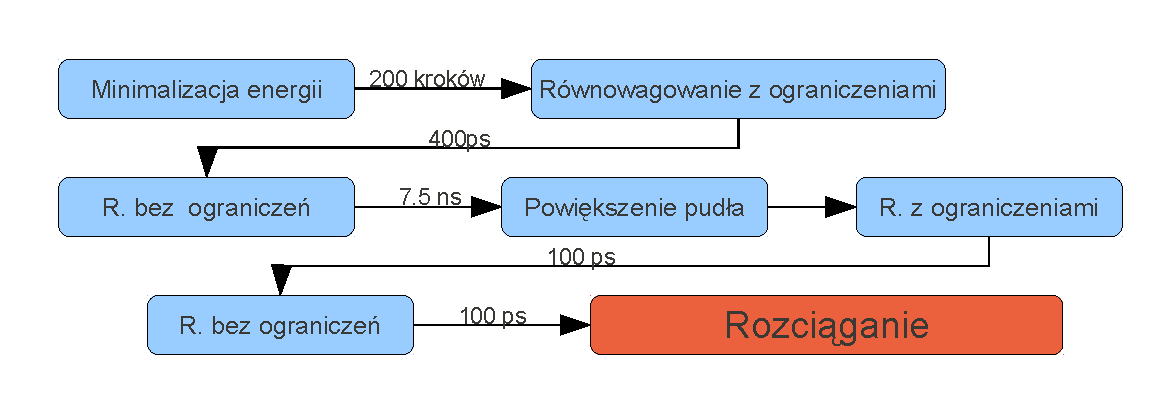
\includegraphics[width=150mm]{./rys/schemat.pdf}
\caption{Schemat przebiegu równowagowania i symulacji.}
\end{centering}
\end{figure}

Przed właściwą symulacją należy przeprowadzić równowagowanie całego układu tak, aby wyeliminować w jak największym stopniu różnice między układem symulowanym, a rzeczywistym. Różnice te wynikają przede wszystkim z faktu, że dysponujemy strukturą krystaliczną, która nie odpowiada w pełni strukturze białka w roztworze, do której dąży się poprzez równowagowanie.


\subsection{Minimalizacja energii}

Pierwszym etapem jest minimalizacja energii całego układu. W wyniku dodawania wody, jonów, a także nieprawidłowości w samej strykturze pliku PDB mogą powstać miejsca, w których atomy znajdują się zbyt blisko siebie lub wręcz nakładają się wiązaniami. Podczas swobodnej symulacji prowadziłoby to do nadania tym atomom znacznie zawyżonych wartości energii kinetycznych, przez co badany układ by się rozpadł. Zjawisko to nazywa się eksplozją układu.

W celu ograniczenia tego efektu prowadzi się minimalizację energii potencjalnej układu. W wyniku tej operacji otrzymuje się układ o jak najmniejszych oddziaływaniach pomiędzy atomami. 

W tym celu utworzono plik z parametrami symulacji \texttt{em.mdp}. Najważniejsze na tym etapie parametry, które służą do kontroli symulacji to wybór integratora czyli algorytmu obliczeniowego oraz nadanie wartości specyficznym dla niego parametrom. W przypadku minimalizacji energii najczęściej wykorzystywanym i najszybszym, ale mało dokładnym algorytmem jest metoda najszybszego spadku. Do jej wyboru służy opcja \texttt{integrator = steep}. Dla tej metody charakterystyczne są parametry:
\begin{itemize}
\item \texttt{emtol} --- Określa maksymalną siłę, poniżej której optymalizacja jest uznana za zakończoną.
\item \texttt{nsteps} --- Maksymalna liczba kroków optymalizacji.
\item \texttt{emstep} --- Krok.
\end{itemize}

Posiadając już plik \texttt{.mdp} wraz ze strukturą oraz topologią należy stworzyć binarny plik wejściowy z rozszerzeniem \texttt{.tpr} dla właściwych obliczeń. Służy do tego program \texttt{grompp}. 

\texttt{grompp -f em -o em -c ions.gro -p topol}

Posiadając już plik \texttt{em.tpr} można uruchomić właściwą symulację. Służy do tego polecenie \texttt{mdrun}. Jednak ze względu na używaną wielowątkowość należy poprzedzić je poleceniem środowiska OpenMPI \texttt{mpirun}.

Do poprawnego działania wymaga ono podania liczby uruchamianych procesów \texttt{-np 16}, od 16 uruchamianych procesów oraz adresów sieciowych komputerów, na których prowadzone będą obliczenia. Można je podać bezpośrednio w linii komend, jednak wygodniej jest umieścić je w pliku, który wskazuje się opcją \texttt{-machinefile}. Na strukturę tego pliku składają się adresy sieciowe lub nazwy hostów komputerów. Opcjonalnie można po spacji podać maksymalną liczbę możliwych do uruchomienia wątków na danym komputerze, w tym przypadku było to 8 \texttt{max-slots=8} oraz liczbę wątków, które mają zostać wykorzystane, \texttt{slots=8}. Po zapisaniu tych linii do pliku \texttt{hosts}, komenda wygląda następująco:

\texttt{mpirun -np 16 -hostfile ./hosts mdrun\_mpi -v -deffnm em}

W wyniku obliczeń uzyskuje się kilka plików z następującymi rozszerzeniami:
\begin{itemize}
\item \texttt{.log} --- Zawiera podsumowanie obliczeń
\item \texttt{.edr} --- Plik z wartościami ciśnienia, temperatury, objętości, wyszczególnionych energii i innymi parametrami w zależności czasowej.
\item \texttt{.trr} --- plik z trajektorią. Przez trajektorię rozumie się położenia atomów oraz ich prędkości w zależności od czasu.
\item \texttt{.gro} --- Struktura po optymalizacji.
\end{itemize}

Korzystając z programu \texttt{g\_energy} można pokazać jak zmieniała się energia potencjalna całego układu wraz z postępem optymalizacji. Na wykresie widać szybki spadek energii potencjalnej na początku minimalizacji oraz niewielkie jej zmiany pod koniec.

\begin{figure}[h]
\begin{centering}
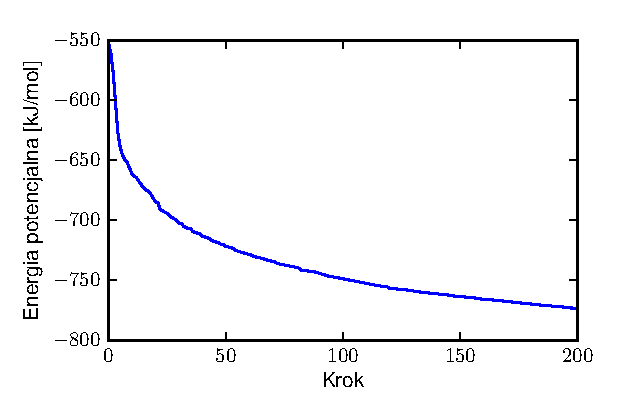
\includegraphics[width=100mm]{./rys/em_pot.pdf}
\caption{Energia potencjalna układu podczas minimalizacji.}
\end{centering}
\end{figure}

\subsection{Równowagowanie rozpuszczalnika}

Kolejnym krokiem w równowagowaniu jest już właściwa symulacja z ograniczeniami nałożonymi na atomy białka tak, by nie zmieniły one swojego położenia. Pozawala to na swobodne rozmieszczenie rozpuszczalnika wraz z jonami wokół białka. Podczas tworzenia topologii przy konwersji z pliku PDB automatycznie tworzony jest plik z ograniczeniami (\texttt{.itp}) dla każdego atomu białka. Jego definicja jest automatycznie dodawania do pliku topologii, jednak domyślnie jest on nieaktywny. Można go aktywować w pliku \texttt{.mdp} dodając linię \texttt{define = -DPOSRES}. Nakłada on na każdy atom białka potencjał harmoniczny ze stałą siłową domyślnie 1000~kJ~mol$^{-1}$~nm$^{-2}$ w każdym z wymiarów przestrzennych. Dzięki temu próba przesunięcia atomu w którymkolwiek kierunku prowadzi do niekorzystnego, wyższego stanu energetycznego układu. Metoda ta ma tę zaletę, że nie prowadzi do całkowitego unieruchomienia wybranych atomów. 

W przypadku właściwej symulacji najczęściej stosowanym integratorem jest \texttt{md}. Tak też jest w tym przypadku. Do najważniejszych parametrów tej opcji należy krok czasowy \texttt{dt} [ps], który po zastosowaniu dalszych algorytmów optymalizacyjnych może być zmniejszony do 2~fs. Mając już ustalony krok czasowy oraz znając czas trwania symulacji można podać jako parametr \texttt{nsteps} liczbę kroków symulacji. W przypadku symulacji trwającej 400~ps liczbę kroków ustalono na 200000. 

Grupa parametrów z prefiksem \texttt{nst} opisuje częstość zapisu wartości takich jak położenia atomów, ich prędkości, energie czy też zwykłe informacje kontrolne na temat symulacji do plików. Zawiera informację co ile kroków parametry te są zapisywane. Ma to wpływ na rozdzielczość późniejszych danych do analizy oraz ilość przestrzeni dyskowej zajmowanej przez zapisaną trajektorię. 

Rozpoczynając symulację należy nadać prędkości początkowe atomom. Służy do tego parametr \texttt{gen\_vel}, który przyjmuje wartości \texttt{yes} albo \texttt{no}. Prędkości dobierane są losowo z rozkładu Maxwella do temperatury podanej w parametrze \texttt{gen\_temp} [K]. Do ustalenia ziarna służy parametr \texttt{gen\_seed}, który ustawiony na \texttt{-1} przybiera wartość automatyczną na podstawie numeru procesu w systemie. Chcąc kontynuować symulację z nowymi parametrami należy pamiętać, by w nowym pliku \texttt{.mdp} ustawić \texttt{gen\_vel} na \texttt{no}. Zapobiegnie to nadaniu nowych prędkości już zrównowagowanemu układowi.

\subsection{Termostat}

Kolejną kwestią jest kontrola temperatury. W wyniku zmniejszonej precyzji obliczeń oraz błędów numerycznych temperatura układu może ulegać znacznym fluktuacjom. Aby tego uniknąć stosuje się algorytmy kontroli stałości temperatury zwane termostatami. W tym przypadku układ równowagowany był do stałej temperatury 300~K. 

Gromacs oferuje do wyboru trzy algorytmy kontroli temperatury (\texttt{berendsen}, \texttt{V-rescale} oraz \texttt{nose-hoover}) określane parametrem \texttt{tcoupl}, gdzie \texttt{no} oznacza brak termostatu. 

Termostat Berendsena stanowi algorytm prostego skalowania prędkości wszystkich cząsteczek w danej grupie. Jako parametr opisujący szybkość doprowadzania układu do zadanej temperatury służy \texttt{tau\_t}, natomiast temperaturę układu, do której się dąży opisuje \texttt{ref\_t}. Aby uniknąć sytuacji, kiedy to większość energii kinetycznej przekazywana jest do rozpuszczalnika, prowadząc do problemu gorącego rozpuszczalnika i zimnej substancji rozpuszczonej zaleca się oddzielne sprzęganie rozpuszczalnika i substancji rozpuszczonej. Grupy te definiuje się parametrem \texttt{tc\_grps} rozdzielając je spacją i podając temperaturę dla każdej z nich.

Termostat Berendsena jest najszybszy, jednak może prowadzić do powstawania błędów, gdyż nie uwzględnia rozkładu statystycznego skalowanych prędkości. Dlatego też w nowszej wersji programu Gromacs zaleca się stosowanie termostatu V-rescale, który jest zmodyfikowanym termostatem Berendsena, w ten sposób,  że uwzględnia poprawny rozkład energii kinetycznej w układzie.

Algorytm Nosé-Hoover jest najwolniejszym, ale też najdokładniejszym z omawianych algorytmów. Pozwala na fluktuację temperatury wokół danej wartości. Jeśli poprzednie dwa termostaty pozawalają na szybkie doprowadzenie układu do pożądanej temperatury, tak ten termostat pozawala na najbardziej wierne jej zachowanie w trakcie symulacji. Jednak w publikacji, na którą się powołano próbując odtworzyć wyniki \cite{1tki} używa się termostatu Berendsena przy temperaturze 300 K oraz stałej sprzęgania $\tau_{T}$=0.1~ps, przez co w symulacjach użyto termostatu V-rescale.

\subsection{Barostat}

Mając ściśle zdefiniowane, stałe początkowe wymiary pudełka traci się kontrolę nad ciśnieniem oraz nad gęstością układu. Aby jak najbardziej zbliżyć symulację do rzeczywistego eksperymentu wprowadzono kontrolę ciśnienia poprzez stosowanie barostatów parametrem \texttt{pcoupl}. Najczęściej stosowanymi dwoma algorytmami są \texttt{berendsen} oraz \texttt{parrinello-rahman}.

Tak jak w przypadku termostatu algorytm Berendsena stanowy szybki i prosty algorytm skalowania, w tym przypadku wymiarów pudełka tak, by doprowadzić ciśnienie układu do pożądanej wartości. Może to prowadzić do błędów, ponieważ nie odwzorowuje prawidłowo układu stałej liczby atomów, ciśnienia i temperatury (NPT). W tym celu lepszym rozwiązaniem jest stosowanie algorytmu Parrinello-Rahmana, jednak należy pamiętać, że działanie tego algorytmu opiera się na oscylacji wokół stałego ciśnienia, co przy początku symulacji z dużej różnicy ciśnień może doprowadzić do nadania atomom niebezpiecznie wysokich prędkości. W omawianej symulacji używa się algorytmu Berendsena.

Do kontroli stałego ciśnienia służą następujące parametry:
\begin{itemize}
\item \texttt{pcoupltype} --- Definiuje rodzaj skalowania pudełka. Najczęściej używanymi są \texttt{isotropic}, gdzie pudełko jest skalowane we wszystkich wymiarach tak samo, \texttt{semiisotropic}, gdzie skalowanie w wymiarze \texttt{x} oraz \texttt{y} jest takie samo, natomiast wymiar \texttt{z} skalowany jest niezależnie (zastosowanie przy symulacji błon lipidowych) oraz \texttt{anisotropic}, gdzie każdy z wymiarów jest skalowany niezależnie, a ponadto skalowane są dodatkowo 3 kierunki diagonalne.
\item \texttt{tau\_p} --- Określa stałą czasową relaksacji $\tau_{p}$ w symulacji określoną jako 1.0~ps.
\item \texttt{ref\_p} --- Określa ciśnienie do którego sprzęgany jest układ. Należy zdefiniować każdy wymiar. Aby w skalowaniu anizotropowym uniknąć skalowania ciśnienia w kierunkach diagonalnych ustala się ciśnienie na 0. Dzięki temu symulowane pudełko nie przekształca się w pudełko trygonalne. W pozostałych wymiarach ciśnienie ustala się na 1.0~bar.
\item \texttt{compressibility} --- Ściśliwość, ustalana w każdym z wymiarów, domyślnie dla wody wynosi 4.5$\times10^{-5}$~bar$^{-1}$. Tak jak w przypadku ciśnienia należy również ustalić 0 dla diagonalnych.
\end{itemize}

Wszystkie parametry dla tego etapu symulacji umieszczono w pliku \texttt{npt\_res.mpd}. Posiadając już ten plik można zastosować polecenia z wcześniejszego etapu. Całość tego symulacji zajęła 48~min~40~s na 16 rdzeniach. 

\subsection{Równowagowanie układu}

Posiadając już strukturę z poprzedniej symulacji można przejść po usunięciu ograniczeń nałożonych na atomy białka do etapu równowagowania całego układu. Dzięki temu struktura krystaliczna białka zbliży się do tej, która występuje w roztworze. 

Po usunięciu ograniczeń położenia atomów białka mogą one w wyniku drgań termicznych ulegać zmianie, w wyniku czego całe białko ulega rotacji i translacji. W wyniku określenia periodyczności układu nie stanowi to problemu podczas równowagowania, jednak przygotowując białko do rozciągania należy to uwzględnić w dalszej symulacji.

Aby mimo wszystko zachować położenie białka w centrum i pozwolić na ustalenie się struktury trzeciorzędowej zbliżonej do tej występującej w roztworze należy usunąć ruch środka ciężkości białka. W tym celu należy zdefiniować w pliku \texttt{mdp} parametr \texttt{comm\_mode} jako \texttt{Linear}, który usuwa ruch translacyjny środka masy, \texttt{Angular}, który usuwa ruch translacyjny jak i rotację cząsteczki lub grupy cząsteczek wokół środka masy lub \texttt{No}.

Tryb \texttt{Linear} może być użyty w obliczeniach wielowątkowych, podczas których zachodzi podział pudełka na obszary, które liczą się oddzielnie (\textit{domain decomposition}), natomiast tryb \texttt{Angular} może być użyty tylko w trybie \textit{particle decomposition}, co oznacza podział nie na obszary, ale na cząsteczki liczone na oddzielnych wątkach. Dlatego też aby przyspieszyć obliczenia nie ustalano parametru \texttt{comm\_mode} w pliku \texttt{.mdp}, dzięki czemu Gromacs automatycznie ustawił go na usuwanie ruchu translacyjnego środka masy umożliwiając tym samym tryb pracy \textit{domain decomposition}.

Równowagowanie prowadzone było przez 7.5~ns, gdzie czas obliczeń na 16 rdzeniach wyniósł 13h 38min 15s.

Do kontroli procesu równowagowania służy obserwacja temperatury i ciśnienia układu, a także RMSD (root-mean-square deviation) czyli pierwiastka ze średniej kwadratów odchyleń położeń atomów od położenia początkowego dla łańcucha głównego białka. Do uzyskania tych danych z obliczonej trajektorii służą polecenia \texttt{g\_rms} oraz \texttt{g\_energy}. Jako parametry wejściowe polecenia te biorą plik \texttt{.tpr} oraz odpowiednio trajektorię \texttt{.trr} lub \texttt{.xtc} oraz plik z danymi o układzie \texttt{.edr}. Na wyjściu otrzymuje się pliki w formacie \texttt{.xvg}, które można otwierać bezpośrednio programem \texttt{xmgrace} lub też jak w tym przypadku poddawać je analizie w innym środowisku, na przykład Python.


\begin{figure}[h]
\begin{centering}
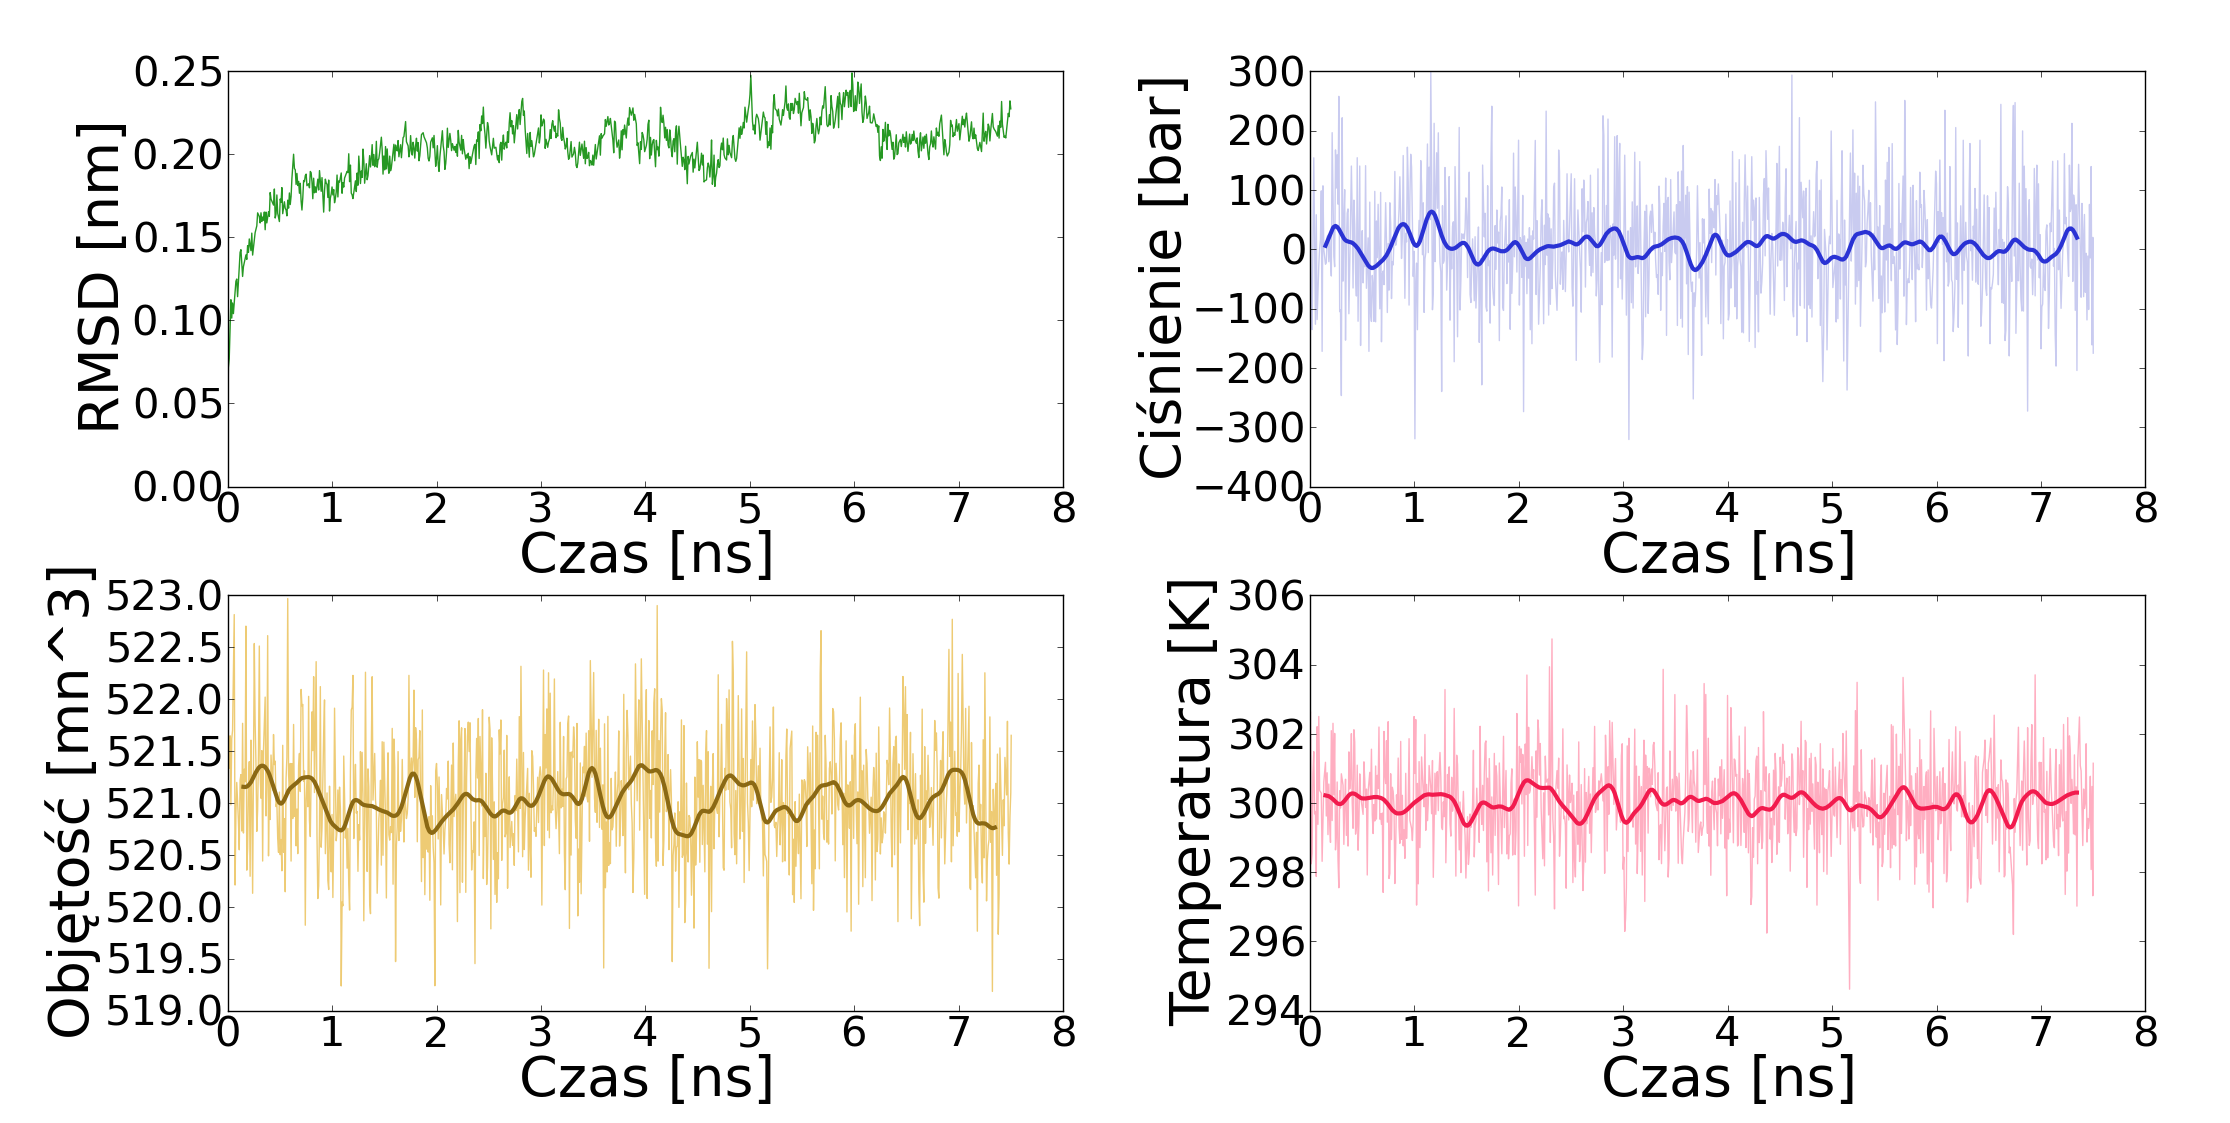
\includegraphics[width=150mm]{./rys/rmsd.png}
\caption{Zmiana RMSD, ciśnienia, objętości i temperatury w czasie podczas równowagowania.}
\end{centering}
\end{figure}


Analiza wykresów p, T i V wskazuje na ustalenie się ich wartości i fluktuację wokół zadanych parametrów, co jest zachowaniem pożądanym. Wykres RMSD także szybko rośnie do pewnego momentu, po czym nie przekracza wartości 0.25 nm, dzięki czemu można domniemywać, że białko osiągnęło strukturę równowagową. Dysponując ograniczonym czasem na wykonanie obliczeń trzeba polegać na założeniu wiarygodności tych danych, którymi się dysponuje, gdyż nigdy nie wiadomo jakim zmianom strukturalnym podlegałoby białko w dalszym czasie.

W wyniku równowagowania bez usuwania rotacji wokół środka ciężkości białka uległo ono obróceniu. Przy symulacji rozciągania jest to niekorzystne, ponieważ należałoby zastosować pudełko sześcienne, które przez zwiększoną objętość powodowałoby zwiększenie czasu obliczeń. Aby tego uniknąć stosuje się pudełko w formie prostopadłościanu o wymiarze zwiększonym tylko w kierunku rozciągania tak, aby pomieścić rozwijane białko. 

W tym celu w dalszym etapie należy białko obrócić tak, by zorientować N i C-koniec białka wzdłuż jednej z osi układu współrzędnych i stworzyć nowe pudełko. 

Służy do tego skrypt napisany w środowisku programistycznym Python (rot.py), który wczytuje plik \texttt{.gro} oraz oblicza kąty pomiędzy wektorem utworzonym pomiędzy dwoma zadanymi atomami, a osiami układu współrzędnych. W przypadku 1TKI atomami tymi były atomy węgla alfa Ile 138 oraz Lys 18. Mając już wartości kątów, korzysta się z polecenia \texttt{editconf} z parametrem \texttt{-rotate}, po którym podaje się kąty w stopniach, o które należy obrócić cząsteczkę wokół osi X Y Z tak, by wybrane wcześniej atomy znalazły się wzdłuż osi Z, po której białko ulega rozciągnięciu. 

Po obrocie pudełka usunięto rozpuszczalnik oraz jony z układu zarówno w pliku \texttt{gro} jak i pliku z topologią. Następnie stworzono nowe pudełko o wymiarach 7.8 x 8.4 x 18.6 nm, dodano rozpuszczalnika oraz jonów według procedury opisanej poprzednio, co w efekcie dało 119587 atomów w układzie. Ponownie równowagowano układ najpierw z ograniczeniami nałożonymi na atomy białka, a następnie bez ograniczeń przez 100~ps. Czas obliczeń na 16 rdzeniach wyniósł odpowiednio 27min 10s oraz 28min 6s. Dzięki tej procedurze równowagowanie białka mogło być przeprowadzone w mniejszym pudełku, a co za tym idzie obliczenia trwały krócej niż miałoby to miejsce przy równowagowaniu przez 7.5~ns przy wymiarach pudełka niezbędnych do symulacji rozciągania. 


\begin{figure}[h]
\begin{centering}
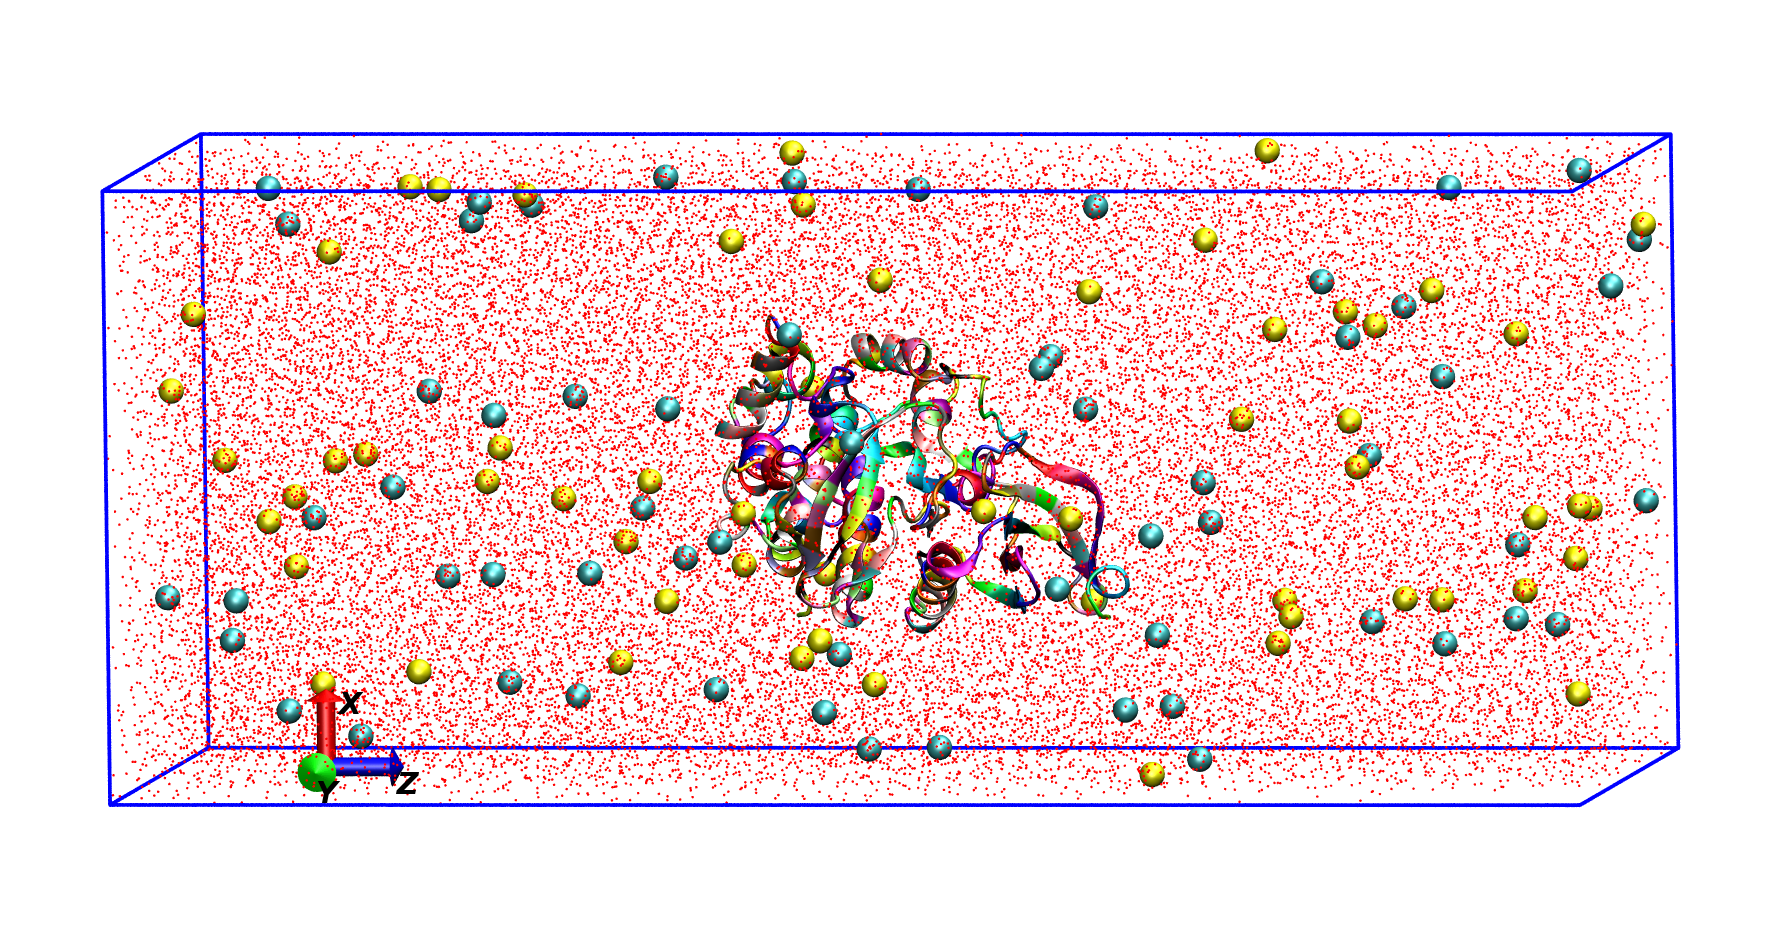
\includegraphics[width=150mm]{./rys/plot.png}
\caption{Wizualizacja symulowanego układu z białkiem, atomami tlenu od wody w kolorze czerwonym, jonami sodu w kolorze żółtym oraz jonami chloru w kolorze jasnoniebieskim.}
\end{centering}
\end{figure}

Posiadając już zrównowagowany układ można było przystąpić do właściwych symulacji rozciągania.

\section{Rozciąganie}

Rozciąganie polega na przyłożeniu wirtualnej sprężyny do środka ciężkości grupy atomów lub tak jak w tym przypadku, do pojedynczych atomów i odsuwaniu jej ze stałą szybkością. Wraz z przemieszczeniem sprężyna o zadanej stałej sprężystości $k$ powoduje powstawanie siły pomiędzy wirtualnym końcem, a danym atomem, co prowadzi do jego przemieszczenia.

Aby przystąpić do rozciągania należało zdefiniować grupy atomów, do których miała zostać przyłożona siła. Służy do tego polecenie \texttt{make\_ndx}, w którym utworzono grupy \texttt{pull} oraz \texttt{stop} z poprzednio opisanych atomów węgla alfa dwóch końcowych aminokwasów. Program \texttt{make\_ndx} posiada własną wewnętrzną składnię. Potrzebne grupy utworzono poleceniami \texttt{r 18 \& a CA} oraz \texttt{r 338 \& a CA}. Przed zapisaniem należało nadać nowo utworzonym grupom nazwy. W wyniku działania tego programu otrzymuje się plik z rozszerzeniem \texttt{.ndx}, który należy uwzględnić przy uruchamianiu \texttt{grompp} opcją \texttt{-n}.

Przy rozciąganiu najdogodniej jest stosować zespół NVE, czyli stałą liczbę cząsteczek, objętość oraz stałą energię układu. Dzięki temu mamy zagwarantowaną stałą energię układu. Wymaga to wyłączenia barostatu oraz termostatu. W tym celu potrzebna jest podwójna precyzja obliczeń. Ponadto aby zapobiec zbytniemu wzrostowi temperatury układu w wyniku obecności zewnętrznej siły, a co za tym idzie pracy, należy zastosować większe pudełko. Powyższe zmiany prowadziłyby do znacznego wydłużenia czasu obliczeń i nie zostały uwzględnione w omawianych symulacjach.

Stosując anizotropowy barostat należy uniemożliwić jego działanie w wymiarze, w którym prowadzi się rozciąganie. Bez tego pudełko ulega odbiegającym od rzeczywistości odkształceniom, mianowicie kurczy się w wymiarze, w którym badana cząsteczka ulega rozciągnięciu.

Za rozciąganie odpowiada sekcja w pliku \texttt{.mdp} zwana \textit{pull code}. Jej parametry przedstawiają się następująco:
\begin{itemize}
\item \textbf{pull} --- Odpowiada za włączenie kodu rozciągania. Opcja \texttt{constant\_force} sprawia, że rozciąganie odbywa się przy stałej sile. W tym przypadku zastosowano opcję \texttt{umbrella}, co pozwala na stosowanie stałej prędkości.
\item \textbf{pull\_geometry} --- \texttt{distance} powoduje rozciąganie wzdłuż wektora łączącego dwie grupy. Opcja \texttt{direction} umożliwia rozciąganie wzdłuż zdefiniowanego wektora. Opcja ta nakłada ograniczenie powodujące, że odległości pomiędzy dwoma rozciąganymi grupami atomów nie mogą przekroczyć połowy wymiaru, w którym zachodzi rozciąganie. Aby uniknąć tego ograniczenia stosuje się opcję \texttt{direction\_periodic}.
\item \textbf{pull\_dim} --- Określa które z wymiarów wektora siły mają być zapisywane. W tym przypadku jest to wartość siły dla osi Z układu współrzędnych.
\item \textbf{pull\_group} --- Zawiera nazwy grup atomów z pliku \texttt{ndx}, które mają zostać poddane rozciąganiu. \texttt{pull\_group0} zawiera definicję grupy odniesienia. W przypadku braku tej definicji za punkt odniesienia bierze się początek układu współrzędnych.
\item \textbf{pull\_vec} --- Definiuje wektor, wzdłuż którego białko ulega rozciąganiu odpowiednio dla każdej z grup poza grupą zerową.
\item \textbf{pull\_rate} --- Określa dla każdej z grup prędkość rozciągania. Podawana jest w pm/ns.
\item \textbf{pull\_k} --- Określa stałą siłową dla każdej z grup w kJ mol$^{-1}$ nm$^{-2}$. W opisywanych symulacjach wynosi 500 kJ mol$^{-1}$ nm$^{-2}$.
\end{itemize}

Symulacje rozciągania dla wszystkich prędkości prowadzone były na 16 rdzeniach, a każda z trajektorii była zapisywana w oddzielnym folderze. Podczas symulacji aktywny był barostat oraz termostat uprzednio używany podczas równowagowania. Rozciąganie odbywało się wzdłuż N-końca oraz C-końca białka. Jako wynik oprócz standardowych plików otrzymano pliki z wartościami siły, \texttt{pullf.xvg}.

\begin{center}
\begin{table}[h]
\centering
  \begin{tabular}{| c | l | l |}
  \hline
  Prędkość [nm/ns] & Czas symulacji [ns] & Czas obliczeń\\
  \hline
  50 & 0.2 & 1h15:55 \\
  10 & 1 & 4h48:31 \\
  5 & 2 & 11h57:22 \\
  2 & 5 & 21h50:17 \\
  0.8 & 10 & 2d7h56:25 \\
  0.4 & 20 & 3d15h07:03\\
  \hline
  \end{tabular}
  \caption{Czasy symulacji dla różnych prędkości rozciągania.}
\end{table}
\end{center}

\begin{lstlisting}[label={kod:polecenia}, caption={Polecenia Gromacsa używane  podczas symulacji podane w kolejności wykonywania}]
pdb2gmx -f hadded.pdb -o tki.gro -ignh -his
editconf -f tki.gro -o box.gro -box 8.8 7.8 7.6 -c
genbox -cp box.gro -cs spc216.gro -o water.gro -p topol.top 

grompp -f em -o ions -p topol -c water
genion -s ions -o ions.gro -p topol.top -nn 29 -np 27
grompp -f em -o em -c ions.gro -p topol
mdrun -v -deffnm em

grompp -f npt_res -o npt_res -c em.gro -p topol
mpirun -np 16 -hostfile ./hosts mdrun_mpi -v -deffnm npt_res
grompp -f npt -o npt -c npt_res.gro -p topol -e npt_res.edr -t npt_res.trr
mpirun -np 16 -hostfile ./hosts mdrun_mpi -v -deffnm npt

#### obrot czasteczki tak, by konce znalazly sie na osi Z
python rot.py
editconf -f npt_rot.gro -o npt_rot.gro -rotate 0 65.662 0
python rot.py
editconf -f npt_rot.gro -o npt_rot.gro -rotate -62.469 0 0
vmd npt_rot.gro
editconf -f npt_rot.gro -o npt_rot.gro -rotate 90 0 0
trjconv -f npt_rot.gro -o npt_large_box.gro -s npt

#### usuniecie z topol.top linii dot. wody i jonow
editconf -f npt_large_box.gro -o npt_large_box.gro -box 7.8 8.4 18.6 -c
genbox -cp npt_large_box.gro -cs spc216.gro -o npt_large_water.gro -p topol.top 
grompp -f em -o npt_large_ions -p topol -c npt_large_water
genion -s npt_large_ions -o npt_large_ions.gro -p topol.top -neutral -c 0.086

grompp -f npt_large_res -o npt_large_res -c npt_large_ions.gro -p topol
mpirun -np 16 -hostfile ./hosts mdrun_mpi -v -deffnm npt_large_res
grompp -f npt_large -o npt_large -c npt_large_res.gro -p topol -e npt_large_res.edr -t npt_large_res.trr
mpirun -np 16 -hostfile ./hosts mdrun_mpi -v -deffnm npt_large

make_ndx -f npt_large -o pull.ndx

cd p50
grompp -f pull.mdp -o pull.tpr -p ../topol.top -c ../npt_large.gro -t ../npt_large -e ../npt_large -n ../pull.ndx -maxwarn
mpirun -np 16  -machinefile ../hosts mdrun_mpi -v -s pull -dlb yes
\end{lstlisting}
